% Options for packages loaded elsewhere
\PassOptionsToPackage{unicode}{hyperref}
\PassOptionsToPackage{hyphens}{url}
%
\documentclass[
]{article}
\usepackage{amsmath,amssymb}
\usepackage{iftex}
\ifPDFTeX
  \usepackage[T1]{fontenc}
  \usepackage[utf8]{inputenc}
  \usepackage{textcomp} % provide euro and other symbols
\else % if luatex or xetex
  \usepackage{unicode-math} % this also loads fontspec
  \defaultfontfeatures{Scale=MatchLowercase}
  \defaultfontfeatures[\rmfamily]{Ligatures=TeX,Scale=1}
\fi
\usepackage{lmodern}
\ifPDFTeX\else
  % xetex/luatex font selection
\fi
% Use upquote if available, for straight quotes in verbatim environments
\IfFileExists{upquote.sty}{\usepackage{upquote}}{}
\IfFileExists{microtype.sty}{% use microtype if available
  \usepackage[]{microtype}
  \UseMicrotypeSet[protrusion]{basicmath} % disable protrusion for tt fonts
}{}
\makeatletter
\@ifundefined{KOMAClassName}{% if non-KOMA class
  \IfFileExists{parskip.sty}{%
    \usepackage{parskip}
  }{% else
    \setlength{\parindent}{0pt}
    \setlength{\parskip}{6pt plus 2pt minus 1pt}}
}{% if KOMA class
  \KOMAoptions{parskip=half}}
\makeatother
\usepackage{xcolor}
\usepackage[margin=1in]{geometry}
\usepackage{color}
\usepackage{fancyvrb}
\newcommand{\VerbBar}{|}
\newcommand{\VERB}{\Verb[commandchars=\\\{\}]}
\DefineVerbatimEnvironment{Highlighting}{Verbatim}{commandchars=\\\{\}}
% Add ',fontsize=\small' for more characters per line
\usepackage{framed}
\definecolor{shadecolor}{RGB}{248,248,248}
\newenvironment{Shaded}{\begin{snugshade}}{\end{snugshade}}
\newcommand{\AlertTok}[1]{\textcolor[rgb]{0.94,0.16,0.16}{#1}}
\newcommand{\AnnotationTok}[1]{\textcolor[rgb]{0.56,0.35,0.01}{\textbf{\textit{#1}}}}
\newcommand{\AttributeTok}[1]{\textcolor[rgb]{0.13,0.29,0.53}{#1}}
\newcommand{\BaseNTok}[1]{\textcolor[rgb]{0.00,0.00,0.81}{#1}}
\newcommand{\BuiltInTok}[1]{#1}
\newcommand{\CharTok}[1]{\textcolor[rgb]{0.31,0.60,0.02}{#1}}
\newcommand{\CommentTok}[1]{\textcolor[rgb]{0.56,0.35,0.01}{\textit{#1}}}
\newcommand{\CommentVarTok}[1]{\textcolor[rgb]{0.56,0.35,0.01}{\textbf{\textit{#1}}}}
\newcommand{\ConstantTok}[1]{\textcolor[rgb]{0.56,0.35,0.01}{#1}}
\newcommand{\ControlFlowTok}[1]{\textcolor[rgb]{0.13,0.29,0.53}{\textbf{#1}}}
\newcommand{\DataTypeTok}[1]{\textcolor[rgb]{0.13,0.29,0.53}{#1}}
\newcommand{\DecValTok}[1]{\textcolor[rgb]{0.00,0.00,0.81}{#1}}
\newcommand{\DocumentationTok}[1]{\textcolor[rgb]{0.56,0.35,0.01}{\textbf{\textit{#1}}}}
\newcommand{\ErrorTok}[1]{\textcolor[rgb]{0.64,0.00,0.00}{\textbf{#1}}}
\newcommand{\ExtensionTok}[1]{#1}
\newcommand{\FloatTok}[1]{\textcolor[rgb]{0.00,0.00,0.81}{#1}}
\newcommand{\FunctionTok}[1]{\textcolor[rgb]{0.13,0.29,0.53}{\textbf{#1}}}
\newcommand{\ImportTok}[1]{#1}
\newcommand{\InformationTok}[1]{\textcolor[rgb]{0.56,0.35,0.01}{\textbf{\textit{#1}}}}
\newcommand{\KeywordTok}[1]{\textcolor[rgb]{0.13,0.29,0.53}{\textbf{#1}}}
\newcommand{\NormalTok}[1]{#1}
\newcommand{\OperatorTok}[1]{\textcolor[rgb]{0.81,0.36,0.00}{\textbf{#1}}}
\newcommand{\OtherTok}[1]{\textcolor[rgb]{0.56,0.35,0.01}{#1}}
\newcommand{\PreprocessorTok}[1]{\textcolor[rgb]{0.56,0.35,0.01}{\textit{#1}}}
\newcommand{\RegionMarkerTok}[1]{#1}
\newcommand{\SpecialCharTok}[1]{\textcolor[rgb]{0.81,0.36,0.00}{\textbf{#1}}}
\newcommand{\SpecialStringTok}[1]{\textcolor[rgb]{0.31,0.60,0.02}{#1}}
\newcommand{\StringTok}[1]{\textcolor[rgb]{0.31,0.60,0.02}{#1}}
\newcommand{\VariableTok}[1]{\textcolor[rgb]{0.00,0.00,0.00}{#1}}
\newcommand{\VerbatimStringTok}[1]{\textcolor[rgb]{0.31,0.60,0.02}{#1}}
\newcommand{\WarningTok}[1]{\textcolor[rgb]{0.56,0.35,0.01}{\textbf{\textit{#1}}}}
\usepackage{graphicx}
\makeatletter
\newsavebox\pandoc@box
\newcommand*\pandocbounded[1]{% scales image to fit in text height/width
  \sbox\pandoc@box{#1}%
  \Gscale@div\@tempa{\textheight}{\dimexpr\ht\pandoc@box+\dp\pandoc@box\relax}%
  \Gscale@div\@tempb{\linewidth}{\wd\pandoc@box}%
  \ifdim\@tempb\p@<\@tempa\p@\let\@tempa\@tempb\fi% select the smaller of both
  \ifdim\@tempa\p@<\p@\scalebox{\@tempa}{\usebox\pandoc@box}%
  \else\usebox{\pandoc@box}%
  \fi%
}
% Set default figure placement to htbp
\def\fps@figure{htbp}
\makeatother
\setlength{\emergencystretch}{3em} % prevent overfull lines
\providecommand{\tightlist}{%
  \setlength{\itemsep}{0pt}\setlength{\parskip}{0pt}}
\setcounter{secnumdepth}{-\maxdimen} % remove section numbering
\renewcommand{\contentsname}{Índice}
\usepackage{booktabs}
\usepackage{longtable}
\usepackage{array}
\usepackage{multirow}
\usepackage{wrapfig}
\usepackage{float}
\usepackage{colortbl}
\usepackage{pdflscape}
\usepackage{tabu}
\usepackage{threeparttable}
\usepackage{threeparttablex}
\usepackage[normalem]{ulem}
\usepackage{makecell}
\usepackage{xcolor}
\usepackage{bookmark}
\IfFileExists{xurl.sty}{\usepackage{xurl}}{} % add URL line breaks if available
\urlstyle{same}
\hypersetup{
  pdftitle={ANALISIS EXPLORATORIO 1 CONCESIONARIO DE AUTOS},
  pdfauthor={Alejandra / Giovanny Porras},
  hidelinks,
  pdfcreator={LaTeX via pandoc}}

\title{ANALISIS EXPLORATORIO 1 CONCESIONARIO DE AUTOS}
\author{Alejandra / Giovanny Porras}
\date{2025-05-24}

\begin{document}
\maketitle

{
\setcounter{tocdepth}{2}
\tableofcontents
}
\subsection{2 Exploracion de datos}\label{exploracion-de-datos}

\begin{enumerate}
\def\labelenumi{\alph{enumi}.}
\tightlist
\item
  Descargar el archivo TABLA\_TALLER.xlsx
\item
  Cargar el archivo de datos en RStudio
\end{enumerate}

\textbf{Rta:} Carga de datos inicial

\begin{Shaded}
\begin{Highlighting}[]
\NormalTok{datos\_base }\OtherTok{\textless{}{-}} \FunctionTok{read\_excel}\NormalTok{(}\StringTok{"D:/MaestriaAnalitica/BasesAnalitica/gitRepository/Proyecto{-}02{-}Autos/BASE/t1fe{-}tabla\_taller.xlsx"}\NormalTok{)}
\FunctionTok{kable}\NormalTok{(}\FunctionTok{head}\NormalTok{(datos\_base, }\DecValTok{10}\NormalTok{,  }\AttributeTok{caption =} \StringTok{"Datos iniciales"}\NormalTok{), }\AttributeTok{format =} \StringTok{"latex"}\NormalTok{, }\AttributeTok{booktabs =} \ConstantTok{TRUE}\NormalTok{) }\SpecialCharTok{\%\textgreater{}\%} 
  \FunctionTok{kable\_styling}\NormalTok{(}\AttributeTok{latex\_options =} \FunctionTok{c}\NormalTok{(}\StringTok{"scale\_down"}\NormalTok{, }\StringTok{"hold\_position"}\NormalTok{))}
\end{Highlighting}
\end{Shaded}

\begin{table}[!h]
\centering
\resizebox{\ifdim\width>\linewidth\linewidth\else\width\fi}{!}{
\begin{tabular}{lllllllrl}
\toprule
PERSONA & EDAD & SEXO & ESTATURA & NIVEL ESCOLAR & MARCA DE AUTO & NUMERO DE HIJOS & SALARIO & MASCOTA\\
\midrule
NA & NA & NA & NA & NA & NA & NA & NA & NA\\
NA & NA & NA & NA & NA & NA & NA & NA & NA\\
PERSONA 1 & 21 & M & 1.54 & MAESTRÍA & AUDI & 0 & 1200000 & SI\\
PERSONA 2 & 26 & F & 1.55 & PROFESIONAL & RENAULT & 5 & 1250000 & NO\\
PERSONA 3 & 30 & F & 1.6 & DOCTORADO & BMW & 2 & 900000 & NO\\
\addlinespace
PERSONA 4 & 31 & f & 1.7 & PROFESIONAL & RENAULT & 2 & 800000 & NO\\
PERSONA 5 & 35 & M & 1.71 & MAESTRÍA & AUDI & 1 & 950000 & NO\\
PERSONA 6 & 65 & M & 1.8 & MAESTRÍA & AUDI & 1 & 2000000 & SI\\
PERSONA 7 & 45 & M & 1.54 & MAESTRÍA & BMW & 1 & 2500000 & NO\\
PERSONA 8 & 42 & F & 1.52 & PROFESIONAL & RENAULT & 1 & 3500000 & SI\\
\bottomrule
\end{tabular}}
\end{table}

\begin{enumerate}
\def\labelenumi{\alph{enumi}.}
\setcounter{enumi}{2}
\tightlist
\item
  Describir brevemente la estructura del conjunto de datos: ¿Cuantos
  clientes estan registrados y que variables incluyen?
\end{enumerate}

\begin{Shaded}
\begin{Highlighting}[]
\NormalTok{no\_datos\_persona }\OtherTok{\textless{}{-}}\NormalTok{ datos\_base }\SpecialCharTok{\%\textgreater{}\%}
  \FunctionTok{filter}\NormalTok{(}\FunctionTok{grepl}\NormalTok{(}\StringTok{"PERSONA"}\NormalTok{, PERSONA)) }\SpecialCharTok{\%\textgreater{}\%}
  \FunctionTok{count}\NormalTok{()}

\NormalTok{cabeceras\_datos }\OtherTok{\textless{}{-}} \FunctionTok{names}\NormalTok{(datos\_base)}
\end{Highlighting}
\end{Shaded}

\textbf{Rta:} El conjunto de datos tiene 60 clientes registrados e
incluyen las varibles PERSONA, EDAD, SEXO, ESTATURA, NIVEL ESCOLAR,
MARCA DE AUTO, NUMERO DE HIJOS, SALARIO, MASCOTA .

\begin{enumerate}
\def\labelenumi{\alph{enumi}.}
\setcounter{enumi}{3}
\tightlist
\item
  Realizar una exploracion rapida utilizando funciones como head(),
  tail(), str(), summary(), \textbf{Rta:} Los ultimos valores son (tail)
\end{enumerate}

\begin{Shaded}
\begin{Highlighting}[]
\NormalTok{ultimos\_datos }\OtherTok{\textless{}{-}} \FunctionTok{tail}\NormalTok{(datos\_base)}
\FunctionTok{kable}\NormalTok{(}\FunctionTok{head}\NormalTok{(ultimos\_datos, }\DecValTok{10}\NormalTok{, }\AttributeTok{caption =} \StringTok{"Datos ultima posicion"}\NormalTok{), }\AttributeTok{format =} \StringTok{"latex"}\NormalTok{, }\AttributeTok{booktabs =} \ConstantTok{TRUE}\NormalTok{) }\SpecialCharTok{\%\textgreater{}\%}\FunctionTok{kable\_styling}\NormalTok{(}\AttributeTok{latex\_options =} \FunctionTok{c}\NormalTok{(}\StringTok{"scale\_down"}\NormalTok{, }\StringTok{"hold\_position"}\NormalTok{))}
\end{Highlighting}
\end{Shaded}

\begin{table}[!h]
\centering
\resizebox{\ifdim\width>\linewidth\linewidth\else\width\fi}{!}{
\begin{tabular}{lllllllrl}
\toprule
PERSONA & EDAD & SEXO & ESTATURA & NIVEL ESCOLAR & MARCA DE AUTO & NUMERO DE HIJOS & SALARIO & MASCOTA\\
\midrule
PERSONA 55 & 30 & F & 1.54 & MAESTRÍA & CHEVROLET & 2 & 2400000 & SI\\
PERSONA 56 & 39 & M & 1.58 & MAESTRÍA & AUDI & 1 & 2600000 & NO\\
PERSONA 57 & 34 & F & 1.6 & DOCTORADO & BMW & 1 & 3500000 & SI\\
PERSONA 58 & 24 & f & 1.7 & PROFESIONAL & RENAULT & 3 & 800000 & SI\\
PERSONA 59 & 20 & M & 1.71 & MAESTRÍA & AUDI & 0 & 850000 & NO\\
\addlinespace
PERSONA 60 & 10 & M & 1.8 & PROFESIONAL & AUDI & 0 & 1000000 & NO\\
\bottomrule
\end{tabular}}
\end{table}

\textbf{Funciones adicionales:}

\begin{Shaded}
\begin{Highlighting}[]
\CommentTok{\#print(str(datos\_base))}
\CommentTok{\#print(dim(datos\_base))}
\CommentTok{\#print(colnames(datos\_base))}
\FunctionTok{print}\NormalTok{(}\FunctionTok{summary}\NormalTok{(datos\_base))}
\end{Highlighting}
\end{Shaded}

\begin{verbatim}
##    PERSONA              EDAD               SEXO             ESTATURA        
##  Length:62          Length:62          Length:62          Length:62         
##  Class :character   Class :character   Class :character   Class :character  
##  Mode  :character   Mode  :character   Mode  :character   Mode  :character  
##                                                                             
##                                                                             
##                                                                             
##                                                                             
##  NIVEL ESCOLAR      MARCA DE AUTO      NUMERO DE HIJOS       SALARIO       
##  Length:62          Length:62          Length:62          Min.   : 800000  
##  Class :character   Class :character   Class :character   1st Qu.:2000000  
##  Mode  :character   Mode  :character   Mode  :character   Median :3450000  
##                                                           Mean   :3286667  
##                                                           3rd Qu.:4700000  
##                                                           Max.   :6500000  
##                                                           NA's   :2        
##    MASCOTA         
##  Length:62         
##  Class :character  
##  Mode  :character  
##                    
##                    
##                    
## 
\end{verbatim}

\begin{enumerate}
\def\labelenumi{\alph{enumi}.}
\setcounter{enumi}{4}
\tightlist
\item
  Identificar si hay datos faltantes y cuantificar cuantos son en total
  y por variable
\end{enumerate}

\begin{Shaded}
\begin{Highlighting}[]
\CommentTok{\#is.na(datos\_base)}
\NormalTok{total\_na }\OtherTok{=}\NormalTok{ datos\_base }\SpecialCharTok{\%\textgreater{}\%}\NormalTok{ is.na }\SpecialCharTok{\%\textgreater{}\%} \FunctionTok{sum}\NormalTok{()  }
\CommentTok{\#Contar NA por columna(variable) }
\NormalTok{na\_por\_columna }\OtherTok{\textless{}{-}} \FunctionTok{colSums}\NormalTok{(}\FunctionTok{is.na}\NormalTok{(datos\_base))}
\NormalTok{tabla\_na }\OtherTok{\textless{}{-}} \FunctionTok{data.frame}\NormalTok{(}
   \AttributeTok{Variable =} \FunctionTok{names}\NormalTok{(na\_por\_columna), }
   \AttributeTok{total\_na =} \FunctionTok{as.vector}\NormalTok{(na\_por\_columna) }
\NormalTok{)}

\CommentTok{\#Contar NA total }
\CommentTok{\#rowSums(is.na(datos\_base))}

\CommentTok{\#Impresion de tabla }
\CommentTok{\#kable(tabla\_na, caption = "Variables faltantes por cuantificar")  \%\textgreater{}\%}
\CommentTok{\#  kable\_styling(full\_width = FALSE, position = "left")}
\end{Highlighting}
\end{Shaded}

\textbf{Rta}: - El numero de total de datos faltantes es \textbf{24} y
por variable son los siguientes:

\begin{longtable}[l]{lr}
\caption{\label{tab:tabla_variables_na}Variables faltantes por cuantificar}\\
\toprule
Variable & total\_na\\
\midrule
PERSONA & 2\\
EDAD & 2\\
SEXO & 3\\
ESTATURA & 2\\
NIVEL ESCOLAR & 3\\
\addlinespace
MARCA DE AUTO & 4\\
NUMERO DE HIJOS & 3\\
SALARIO & 2\\
MASCOTA & 3\\
\bottomrule
\end{longtable}

\begin{itemize}
\tightlist
\item
  Analisis: Hay problemas de datos en todas las variables sera
  importante discriminar cada caso
\end{itemize}

\begin{enumerate}
\def\labelenumi{\alph{enumi}.}
\setcounter{enumi}{5}
\tightlist
\item
  Comentar sobre los posibles problemas en los datos:
\end{enumerate}

\textbf{Filas vacías al inicio del archivo:} - Las dos primeras filas
están vacías o no contienen datos válidos.

\textbf{Inconsistencias categóricas:}

\begin{itemize}
\tightlist
\item
  Variabilidad en la codificación de la variable SEXO, con valores como
  f, mujer, hombre, nan o minúsculas inconsistentes.
\item
  Formatos no estandarizados en NIVEL ESCOLAR, como el uso de PhD en
  lugar de DOCTORADO.
\item
  Uso de minúsculas en valores de MARCA DE AUTO, como renault.
\end{itemize}

\textbf{Valores faltantes:}

\begin{itemize}
\tightlist
\item
  Algunas filas tienen múltiples variables vacías, como en el caso de la
  PERSONA 24.
\end{itemize}

\textbf{Valores extremos o anómalos (outliers):}

\begin{itemize}
\tightlist
\item
  PERSONA 31: valor de ESTATURA = 3.45 m, fuera del rango fisiológico
  normal.
\item
  PERSONA 33: valor de NUMERO DE HIJOS = 54, ampliamente fuera del
  promedio observado (3.03).
\end{itemize}

\newpage

\subsection{3 Análisis de la variable Marca ``Marca de
auto''.}\label{anuxe1lisis-de-la-variable-marca-marca-de-auto.}

\begin{enumerate}
\def\labelenumi{\alph{enumi}.}
\tightlist
\item
  Evaluar la variable \textbf{``MARCA DE AUTO''} y determinar si hay
  faltantes.
\end{enumerate}

\begin{Shaded}
\begin{Highlighting}[]
\NormalTok{ data\_na\_marca\_autos }\OtherTok{\textless{}{-}} \FunctionTok{sum}\NormalTok{(}\FunctionTok{is.na}\NormalTok{(datos\_base}\SpecialCharTok{$}\StringTok{\textasciigrave{}}\AttributeTok{MARCA DE AUTO}\StringTok{\textasciigrave{}}\NormalTok{))}
\end{Highlighting}
\end{Shaded}

\textbf{Rta:} Se tratan datos faltantes y se encuentran un total de
\textbf{4}; se realiza tratamiento de datos remplazando los
``na''/``NA'' a ``SIN\_CONFIRMAR'', se convierte todo mayúsculas.

\begin{Shaded}
\begin{Highlighting}[]
 \CommentTok{\#Tratamiento datos MARCA DE AUTOS }
 \CommentTok{\#Eliminar columna 1, 2 }
\NormalTok{ datos\_base }\OtherTok{\textless{}{-}}\NormalTok{ datos\_base[}\SpecialCharTok{{-}}\FunctionTok{c}\NormalTok{(}\DecValTok{1}\NormalTok{,}\DecValTok{2}\NormalTok{), ]}
 \CommentTok{\#Datos Eliminados}
\NormalTok{ na\_marca\_autos }\OtherTok{\textless{}{-}} \FunctionTok{sum}\NormalTok{(}\FunctionTok{is.na}\NormalTok{(datos\_base}\SpecialCharTok{$}\StringTok{\textasciigrave{}}\AttributeTok{MARCA DE AUTO}\StringTok{\textasciigrave{}}\NormalTok{)) }
 \CommentTok{\# PERSONA 13, 32, 49, NA y datos vacios }
\NormalTok{ datos\_base}\SpecialCharTok{$}\StringTok{\textasciigrave{}}\AttributeTok{MARCA DE AUTO}\StringTok{\textasciigrave{}}\NormalTok{[}\FunctionTok{is.na}\NormalTok{(datos\_base}\SpecialCharTok{$}\StringTok{\textasciigrave{}}\AttributeTok{MARCA DE AUTO}\StringTok{\textasciigrave{}}\NormalTok{) }\SpecialCharTok{|}\NormalTok{ datos\_base}\SpecialCharTok{$}\StringTok{\textasciigrave{}}\AttributeTok{MARCA DE AUTO}\StringTok{\textasciigrave{}} \SpecialCharTok{==} \StringTok{"NA"}\NormalTok{] }\OtherTok{\textless{}{-}} \StringTok{"SIN\_CONFIRMAR"}
 \CommentTok{\# PERSONA 39 cambia FOR A FORD }
\NormalTok{ datos\_base}\SpecialCharTok{$}\StringTok{\textasciigrave{}}\AttributeTok{MARCA DE AUTO}\StringTok{\textasciigrave{}}\NormalTok{[ datos\_base}\SpecialCharTok{$}\StringTok{\textasciigrave{}}\AttributeTok{MARCA DE AUTO}\StringTok{\textasciigrave{}} \SpecialCharTok{==} \StringTok{"FOR"}\NormalTok{] }\OtherTok{\textless{}{-}} \StringTok{"FORD"}
 \CommentTok{\# PERSONA 40 cambia BWM A BMW }
\NormalTok{ datos\_base}\SpecialCharTok{$}\StringTok{\textasciigrave{}}\AttributeTok{MARCA DE AUTO}\StringTok{\textasciigrave{}}\NormalTok{[ datos\_base}\SpecialCharTok{$}\StringTok{\textasciigrave{}}\AttributeTok{MARCA DE AUTO}\StringTok{\textasciigrave{}} \SpecialCharTok{==} \StringTok{"BWM"}\NormalTok{] }\OtherTok{\textless{}{-}} \StringTok{"BMW"}
 \CommentTok{\# PERSONA 36 cambio a mayuscula marca }
\NormalTok{ datos\_base}\SpecialCharTok{$}\StringTok{\textasciigrave{}}\AttributeTok{MARCA DE AUTO}\StringTok{\textasciigrave{}} \OtherTok{\textless{}{-}} \FunctionTok{toupper}\NormalTok{(datos\_base}\SpecialCharTok{$}\StringTok{\textasciigrave{}}\AttributeTok{MARCA DE AUTO}\StringTok{\textasciigrave{}}\NormalTok{)}
\end{Highlighting}
\end{Shaded}

\begin{enumerate}
\def\labelenumi{\alph{enumi}.}
\setcounter{enumi}{1}
\tightlist
\item
  Crear una tabla de frecuencias para entender la popularidad de las
  diferentes marcas entre los cliente.
\end{enumerate}

\textbf{Rta: }En la tabla de frecuencias se observa que las marcas más
populares son AUDI, CHEVROLET, RENAULT y BMW. Los tres usuarios que no
tienen la categoría ``\,``SIN\_CONFIRMAR''\,'' se identificaron como
personas a partir de 50 años.

\begin{tabular}{lr}
\toprule
MARCA DE AUTO & Frecuencia\\
\midrule
AUDI & 13\\
RENAULT & 13\\
BMW & 12\\
CHEVROLET & 12\\
FORD & 7\\
\addlinespace
SIN\_CONFIRMAR & 3\\
\bottomrule
\end{tabular}

\begin{enumerate}
\def\labelenumi{\alph{enumi}.}
\setcounter{enumi}{2}
\tightlist
\item
  Generar gráficos de barras y de tortas para visualizar la distribución
  de las marcas de autos y proporcionar una interpretación.
\end{enumerate}

\textbf{Rta: } - Se identifica que las marcas de vehículos preferidas
por los clientes del concesionario son \textbf{AUDI} y \textbf{RENAULT};
se observa una segmentación igual por pares entre las entre AUDI/RENAULT
y CHEVROLET/BMW

\begin{itemize}
\tightlist
\item
  La preferencia de vehículos esta distribuida entre 4 marcas que suman
  83\% de la muestra, estas cuatro marcas a su vez representan dos
  segmentos que se reparten en el mismo porcentaje 21\%/21\% y
  20\%/20\%.
\end{itemize}

\begin{Shaded}
\begin{Highlighting}[]
\NormalTok{ grafico\_barras }\SpecialCharTok{+}\NormalTok{ grafico\_pastel   }\SpecialCharTok{+} \FunctionTok{plot\_layout}\NormalTok{(}\AttributeTok{widths =} \FunctionTok{c}\NormalTok{(}\DecValTok{4}\NormalTok{, }\FloatTok{4.5}\NormalTok{))}
\end{Highlighting}
\end{Shaded}

\pandocbounded{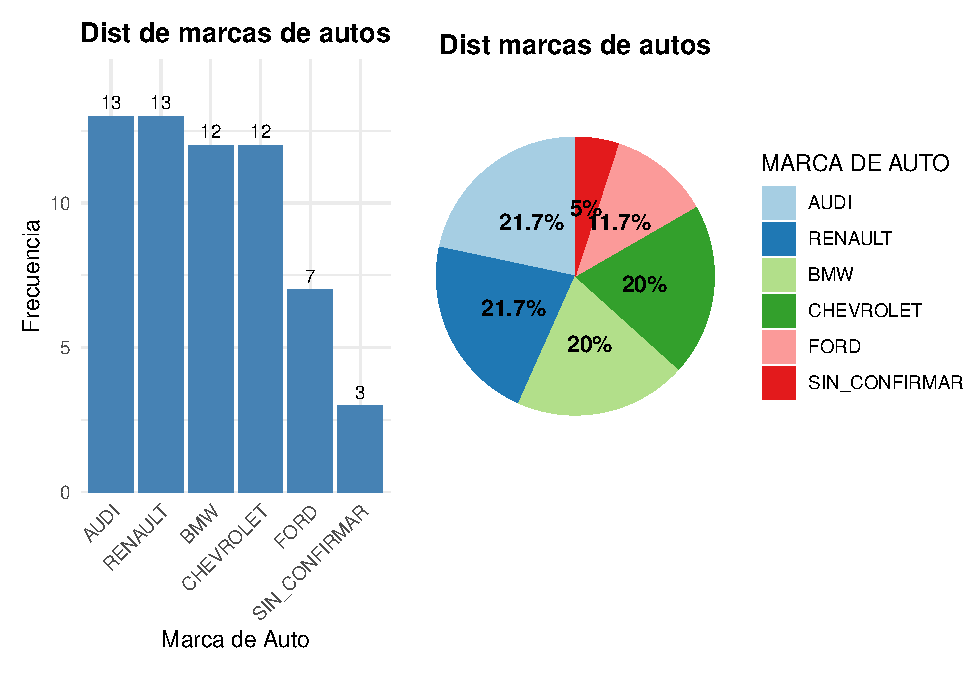
\includegraphics[keepaspectratio]{Reporte01-autors_files/figure-latex/unnamed-chunk-4-1.pdf}}

\begin{enumerate}
\def\labelenumi{\alph{enumi}.}
\setcounter{enumi}{3}
\tightlist
\item
  Concluir cuál es la marca de auto más popular entre los clientes.
\end{enumerate}

\textbf{Rta: } Se concluyen que AUDI y RENAULT son las marcas lideres
con una distribución uniforme en el los clientes del concesionario en un
porcentaje del 21.7 entre ambas ocupan el 42.4\%.

\newpage

\subsection{4 Análisis de la variable
``Edad''.}\label{anuxe1lisis-de-la-variable-edad.}

\begin{enumerate}
\def\labelenumi{\alph{enumi}.}
\tightlist
\item
  Verificar si la variable ``EDAD'' está correctamente importada como
  tipo numérico.
\end{enumerate}

\textbf{Rta:} La variable edad es de tipo \textbf{caracter} sin embargo
su naturaleza es de tipo Cuantitativa discreta para este conjunto de
datos por este motivo se va a relizar la conversión a \textbf{numeric}
en la sección dedicada a normalización de datos.

\begin{Shaded}
\begin{Highlighting}[]
\FunctionTok{summary}\NormalTok{(datos\_base}\SpecialCharTok{$}\NormalTok{EDAD)}
\end{Highlighting}
\end{Shaded}

\begin{verbatim}
##    Length     Class      Mode 
##        60 character character
\end{verbatim}

\begin{enumerate}
\def\labelenumi{\alph{enumi}.}
\setcounter{enumi}{1}
\tightlist
\item
  Identificar cualquier valor incorrecto (por ejemplo, texto en lugar de
  números) y corrija los errores.
\end{enumerate}

\textbf{Rta: }Se encuentran datos incosistententes por formato y
\textbf{NA} se imputa la media para ambos casos, para el caso de
aoutfillers se trabaja con el datos atipico de 10 años para la persona
que tenia una edad de 10 años imputando la media.

\begin{Shaded}
\begin{Highlighting}[]
\CommentTok{\#TRATAMIENTO DE DATOS }
\CommentTok{\#Agrega NA a los datos que no se pueden convertir a numerico }
\NormalTok{datos\_base}\SpecialCharTok{$}\NormalTok{EDAD }\OtherTok{\textless{}{-}} \FunctionTok{as.numeric}\NormalTok{(datos\_base}\SpecialCharTok{$}\NormalTok{EDAD)}
\end{Highlighting}
\end{Shaded}

\begin{verbatim}
## Warning: NAs introducidos por coerción
\end{verbatim}

\begin{Shaded}
\begin{Highlighting}[]
\CommentTok{\#Lista las personas que tienen problemas 24 y 28}
\NormalTok{datos\_base[}\FunctionTok{is.na}\NormalTok{(datos\_base}\SpecialCharTok{$}\NormalTok{EDAD), }\FunctionTok{c}\NormalTok{(}\StringTok{"PERSONA"}\NormalTok{, }\StringTok{"EDAD"}\NormalTok{)]}
\end{Highlighting}
\end{Shaded}

\begin{verbatim}
## # A tibble: 2 x 2
##   PERSONA     EDAD
##   <chr>      <dbl>
## 1 PERSONA 24    NA
## 2 PERSONA 28    NA
\end{verbatim}

\begin{Shaded}
\begin{Highlighting}[]
\CommentTok{\#Se realiza la imputacion de la media a los datos con problema}
\NormalTok{datos\_base}\SpecialCharTok{$}\NormalTok{EDAD[}\FunctionTok{is.na}\NormalTok{(datos\_base}\SpecialCharTok{$}\NormalTok{EDAD)] }\OtherTok{\textless{}{-}} \FunctionTok{median}\NormalTok{(datos\_base}\SpecialCharTok{$}\NormalTok{EDAD, }\AttributeTok{na.rm =} \ConstantTok{TRUE}\NormalTok{)}
\CommentTok{\#summary(datos\_base$EDAD)}
\CommentTok{\#Datos atipicos}
\NormalTok{rango\_edad }\OtherTok{\textless{}{-}} \FunctionTok{range}\NormalTok{(datos\_base}\SpecialCharTok{$}\NormalTok{EDAD, }\AttributeTok{na.rm =} \ConstantTok{TRUE}\NormalTok{)}
\CommentTok{\# Mostrar dos gráficos uno al lado del otro}
\FunctionTok{par}\NormalTok{(}\AttributeTok{mfrow =} \FunctionTok{c}\NormalTok{(}\DecValTok{1}\NormalTok{, }\DecValTok{2}\NormalTok{))  }\CommentTok{\# 1 fila, 2 columnas}
\FunctionTok{boxplot}\NormalTok{(datos\_base}\SpecialCharTok{$}\NormalTok{EDAD, }\AttributeTok{main =} \StringTok{"Outliers en Edad"}\NormalTok{, }\AttributeTok{ylab =} \StringTok{"Edad"}\NormalTok{, }\AttributeTok{col =} \StringTok{"lightblue"}\NormalTok{, }\AttributeTok{ylim=}\NormalTok{rango\_edad )}
\NormalTok{datos\_base}\SpecialCharTok{$}\NormalTok{EDAD[datos\_base}\SpecialCharTok{$}\NormalTok{EDAD }\SpecialCharTok{==} \DecValTok{10}\NormalTok{] }\OtherTok{\textless{}{-}} \FunctionTok{median}\NormalTok{(datos\_base}\SpecialCharTok{$}\NormalTok{EDAD, }\AttributeTok{na.rm =} \ConstantTok{TRUE}\NormalTok{)}
\NormalTok{rango\_edad }\OtherTok{\textless{}{-}} \FunctionTok{range}\NormalTok{(datos\_base}\SpecialCharTok{$}\NormalTok{EDAD, }\AttributeTok{na.rm =} \ConstantTok{TRUE}\NormalTok{)}
\FunctionTok{boxplot}\NormalTok{(datos\_base}\SpecialCharTok{$}\NormalTok{EDAD, }\AttributeTok{main =} \StringTok{"Outliers ajustados en Edad"}\NormalTok{, }\AttributeTok{ylab =} \StringTok{"Edad"}\NormalTok{, }\AttributeTok{col =} \StringTok{"lightgreen"}\NormalTok{, }\AttributeTok{ylim=}\NormalTok{rango\_edad)}
\end{Highlighting}
\end{Shaded}

\pandocbounded{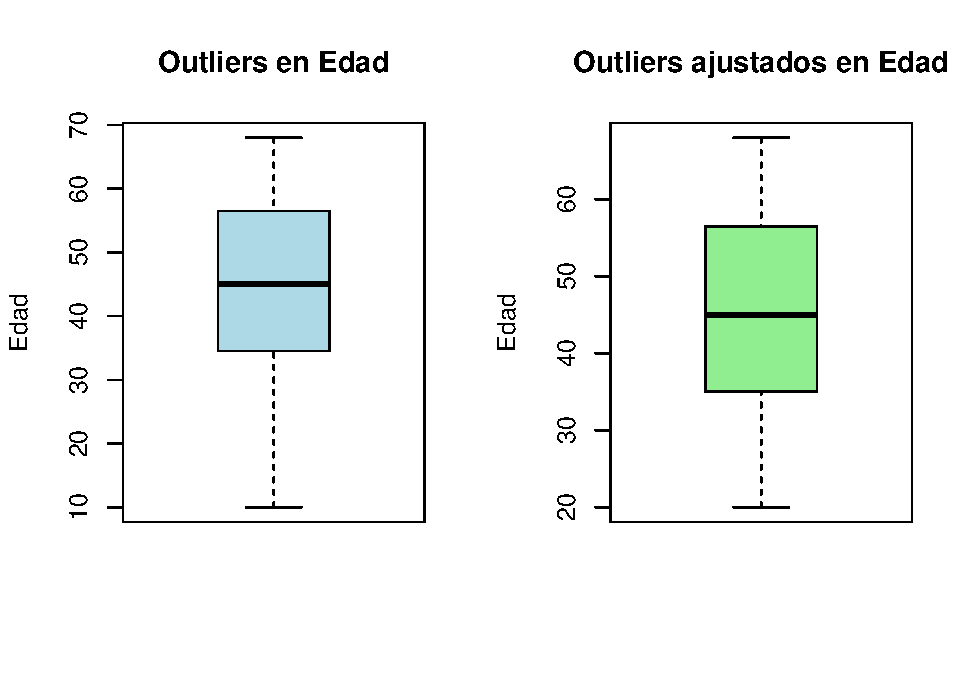
\includegraphics[keepaspectratio]{Reporte01-autors_files/figure-latex/tratamiento_datos_edad-1.pdf}}

\begin{Shaded}
\begin{Highlighting}[]
\CommentTok{\# Restaurar configuración gráfica a 1 gráfico por figura (opcional)}
\FunctionTok{par}\NormalTok{(}\AttributeTok{mfrow =} \FunctionTok{c}\NormalTok{(}\DecValTok{1}\NormalTok{, }\DecValTok{1}\NormalTok{))}
\CommentTok{\#outliers \textless{}{-} boxplot.stats(datos\_base$EDAD)$out ? No funciono }
\end{Highlighting}
\end{Shaded}

\begin{enumerate}
\def\labelenumi{\alph{enumi}.}
\setcounter{enumi}{2}
\tightlist
\item
  Realizar un histograma de la variable edad y describir qué patrones se
  observan entre los clientes (ej. ¿son jóvenes? ¿predomina alguna
  franja de edad?)
\end{enumerate}

\textbf{Rta: } - La franja de edad en la que se presentan mayor numero
de clientes de concesionario estan en la edad de los 40 a los 45 años. -
La franja de 55 a 65 años presenta una gran numeros de clientes - El
sector joven no presenta una alta concentracion con excepcion de la
franja de los 25-30 años

\begin{Shaded}
\begin{Highlighting}[]
\CommentTok{\# Histograma básico para la variable EDAD}
\FunctionTok{ggplot}\NormalTok{(datos\_base, }\FunctionTok{aes}\NormalTok{(}\AttributeTok{x =}\NormalTok{ EDAD)) }\SpecialCharTok{+}
  \FunctionTok{geom\_histogram}\NormalTok{(}\AttributeTok{binwidth =} \DecValTok{5}\NormalTok{,            }\CommentTok{\# Ancho de cada barra: 5 años}
                 \AttributeTok{fill =} \StringTok{"skyblue"}\NormalTok{,        }\CommentTok{\# Color de relleno}
                 \AttributeTok{color =} \StringTok{"white"}\NormalTok{,         }\CommentTok{\# Color del borde}
                 \AttributeTok{boundary =} \DecValTok{0}\NormalTok{) }\SpecialCharTok{+}          \CommentTok{\# Alinear límites en múltiplos de 5}
  \FunctionTok{labs}\NormalTok{(}\AttributeTok{title =} \StringTok{"Distribución de Edades"}\NormalTok{,}
       \AttributeTok{x =} \StringTok{"Edad (años)"}\NormalTok{,}
       \AttributeTok{y =} \StringTok{"Frecuencia"}\NormalTok{) }\SpecialCharTok{+}
  \FunctionTok{theme\_minimal}\NormalTok{()}
\end{Highlighting}
\end{Shaded}

\pandocbounded{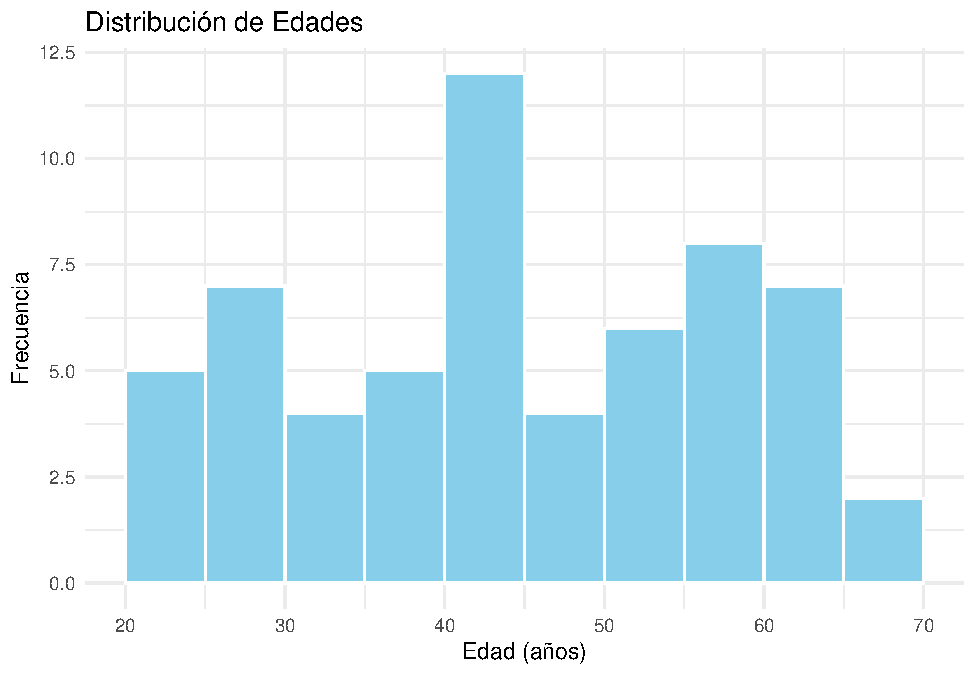
\includegraphics[keepaspectratio]{Reporte01-autors_files/figure-latex/unnamed-chunk-6-1.pdf}}

\end{document}
